\section{Motivation}
\begin{frame}
    Guazzelli et al examined a dilute suspension of rod-like particles influenced by gravity.
\begin{columns}
	\begin{column}{0.5\textwidth}
		\begin{itemize}
			\item In an initially homogeneous suspension, rod-like particles form clusters where they are denser.
			\item The clusters create downward flows balanced by upward flows.
			\item Particles in a cluster mostly align with gravity, occasionally flipping.
		\end{itemize}
	\end{column}
	\begin{column}{0.5\textwidth}
		\begin{figure}[H]
			\centering
			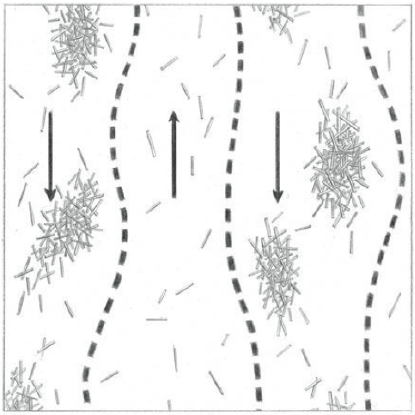
\includegraphics[scale=0.5]{Bilder/Bild_Particles}
		\end{figure}
	\end{column}
\end{columns}
\end{frame}

\begin{frame}{Mathematical Model for the Sedimentation of Rod-Like Particles}
	\scriptsize
\text{Coupling of a kinetic Smoluchowski equation with Navier-Stokes equation}
\begin{align*}
	\textcolor{blue}{\partial_t f}+ \textcolor{red}{\nabla_{\boldsymbol{x}} \cdot(\boldsymbol{u} f)} & +\textcolor{blue}{\nabla_{\boldsymbol{n}} \cdot\left(P_{\boldsymbol{n}^{\perp}} \nabla_{\boldsymbol{x}} \boldsymbol{u} \boldsymbol{n} f\right)}- \textcolor{red}{\nabla_{\boldsymbol{x}} \cdot\left((I+\boldsymbol{n} \otimes \boldsymbol{n}) e_3 f\right)} \\
	& =\textcolor{blue}{D_r \Delta_n f}+\gamma \nabla_{\boldsymbol{x}} \notag \cdot(I+\boldsymbol{n} \otimes \boldsymbol{n}) \nabla_{\boldsymbol{x}} f, \\
	\sigma & =\int_{S^{d-1}}(\text{d} \; \boldsymbol{n} \otimes \boldsymbol{n}-I) f d \boldsymbol{n},  \\
	\operatorname{Re}\left(\partial_t \boldsymbol{u}+\left(\boldsymbol{u} \cdot \nabla_{\boldsymbol{x}}\right) \boldsymbol{u}\right) & =\Delta_{\boldsymbol{x}} \boldsymbol{u}-\nabla_{\boldsymbol{x}} p+\delta \gamma \nabla_{\boldsymbol{x}} \cdot \sigma-\delta \int_{S^{d-1}} f d \boldsymbol{n} \, e_3, \\
	\nabla_{\boldsymbol{x}} \cdot \boldsymbol{u} & =0,
\end{align*}
where $f = f(\boldsymbol{x}, t, \boldsymbol{n}), \boldsymbol{x} \in \mathbb{R}^3 , \boldsymbol{n} \in  S^2$ is a density distribution function of particle orientation. $D_r, \gamma, \delta$ and $Re$ are non-dimensional parameters.
\begin{beamercolorbox}[sep=1em,wd=\linewidth,right]{}
	\tiny{Helzel $\&$ Tzavaras, 2017}
\end{beamercolorbox}
Here we consider the case $\gamma = 0$.
\end{frame}


\begin{frame}{Status of Project}
	\scriptsize
    \begin{block}{So far...}
    	\begin{itemize}
    		\item  Investigate hierarchy of moment equations for simplified model with \textcolor{cyan}{$f$ on $S^1$}
    		\begin{itemize}
    		\item <1->  Transform high dimensional scalar PDE (in space and orientation) into a lower dimensional system of moment equations (in
    		space)
    	   \item <2-> Investigate accuracy of moment closure system
    	    \end{itemize}
    	\end{itemize}
       	   Dahm, Helzel, MMS 2022, Dahm, Giesselmann, Helzel, JCP 2024
    \end{block}
	\begin{block}{Now}
		\begin{itemize}
			\item <3-> Derive and approximate hierarchies of moment equations for the coupled kinetic-fluid model with \textcolor{cyan}{$f$ on $S^2$}.
		\end{itemize}
	\end{block}
\end{frame}
%%%%%%%%%%%%%%%%%%%%%%%%%%%%%%%%%%%%%%%%%%%%%%%%%%%%%%
\begin{comment}
\begin{frame}{Spectral method}
	\scriptsize
	Consider the drift-diffusion equation
	\begin{align}
		\textcolor{blue}{\partial_t f}+ \textcolor{gray!80}{\nabla_{\boldsymbol{x}} \cdot(\boldsymbol{u} f)} & +\textcolor{blue}{\nabla_{\boldsymbol{n}} \cdot\left(P_{\boldsymbol{n}^{\perp}} \nabla_{\boldsymbol{x}} \boldsymbol{u} \boldsymbol{n} f\right)}-\textcolor{gray!80}{\nabla_{\boldsymbol{x}} \cdot\left((I+\boldsymbol{n} \otimes \boldsymbol{n}) e_3 f\right)} \notag \\
		& = \textcolor{blue}{D_r \Delta_n f}+\textcolor{gray!80}{\gamma \nabla_{\boldsymbol{x}} \cdot(I+\boldsymbol{n} \otimes \boldsymbol{n}) \nabla_{\boldsymbol{x}} f} \label{SmochEq_kurz}
	\end{align}
	with externally imposed velocity gradient $\nabla_x. \boldsymbol{u}_{\mathrm{ext}}$\\
	\vspace{12pt}
	\pause
	In spherical coordinates
	\begin{align}
		\underbrace{\sin \theta \partial_t f}_{[1]} + \underbrace{\partial_\phi\left(a(\phi, \theta) f\right)+\partial_\theta\left(b(\phi, \theta) f\right)}_{[2]} = \underbrace{D_r \left(\partial_\phi\left(\frac{1}{\sin \theta} \partial_\phi f\right)+\partial_\theta\left(\sin \theta \partial_\theta f\right)\right)}_{[3]}, \label{Smoch_S2}
	\end{align}	
	with $\phi \in [0, 2 \pi]$ and $\theta \in [0, \pi]$.\\
	\vspace{12pt}
	\pause
  Ansatz for our \textcolor{cyan}{spectral method}
\begin{align}
	f(x,t,\phi, \theta) \approx f_0(x,t) \cdot P_0^0 + \sum_{n=1}^{N} \sum_{k=-2n}^{2n} c^k_{2n}(x,t) \cdot P^k_{2n}(\phi, \theta), \label{ansatz}
\end{align}
where $P^k_{2n}(\phi, \theta)$ are harmonic polynomial basis functions.  %, i.e. are eigenfunctions of Laplace Beltrami operator.
\end{frame}

\begin{frame}{Example}
	\scriptsize
	For $N=1$ we obtain
	\begin{equation}
		\left(\begin{array}{c}
			f_0(t) \\
			c_2^{-2}(t) \\
			c_2^{-1}(t) \\
			c_2^0(t) \\
			c_2^1(t) \\
			c_2^2(t)
		\end{array}\right)^{\prime} - A \cdot
		\left(\begin{array}{c}
			f_0(t) \\
			c_2^{-2}(t) \\
			c_2^{-1}(t) \\
			c_2^0(t) \\
			c_2^1(t) \\
			c_2^2(t)
		\end{array}\right) = -6 D_r \cdot
		\left(\begin{array}{c}
			0 \\
			c^{-2}_2(t) \\
			c_2^{-1}(t) \\
			c_2^0(t) \\
			c_2^1(t) \\
			c_2^2(t)
		\end{array}\right),
	\end{equation}
\end{frame}

\begin{frame}
	where the matrix $A$ has the form \\
	\vspace{8pt}
	\begin{multline*}
		\resizebox{\textwidth}{!}{%
			\(
			\begin{pmatrix}
				\vspace{12pt}
				0 & 0 & 0 & 0 & 0 & 0 \\
				\vspace{12pt}
				\frac{1}{5}\sqrt{15}(u_x-v_y) & \frac{1}{7}(u_x+v_y-2w_z) & \frac{1}{7}(-5u_z+2w_x) & \frac{1}{7}\sqrt{3}(-u_x+v_y) & \frac{1}{7}(5v_z-2w_y) &  (u_y -v_x) \\
				\vspace{12pt}
				\frac{1}{5}\sqrt{15}(-u_z-w_x) & \frac{1}{7}(2u_z-5w_x) & \frac{1}{7}(u_x-2v_y+w_z) & \frac{1}{7}\sqrt{3}(-4u_z+3w_x) & \frac{1}{7}(5u_y-2v_x) &  \frac{1}{7} \left(2v_z-5w_y\right) \\
				\vspace{12pt}
				\frac{1}{5}\sqrt{5}(-u_x-v_y+2w_z) & \frac{1}{7}\sqrt{3}(-u_x+v_y) & \frac{1}{7}\sqrt{3}(3u_z-4w_x) & \frac{1}{7}(-u_x-v_y+2w_z) & \frac{1}{7}\sqrt{3}(-3v_z-4w_y) & \frac{1}{7} \sqrt{3}\left(-u_y-v_x\right) \\
				\vspace{12pt}
				\frac{1}{5}\sqrt{15}(-v_z-w_y) & \frac{1}{7}(-2v_z+5w_y) & \frac{1}{7}(-2u_y+5v_x) & \frac{1}{7}\sqrt{3}(-4v_z+3w_y) & \frac{1}{7}(-2u_x+v_y+w_z) &  \frac{1}{7} \left(2u_z-5w_x\right)\\
				\vspace{12pt}
				\frac{1}{5}\sqrt{15}(u_y+v_x) & (-u_y+v_x) & \frac{1}{7}(-5v_z+2w_y) & \frac{1}{7}\sqrt{3}(-u_y-v_x) & \frac{1}{7}(-5u_z+2w_x) & \frac{1}{7} \left(u_x+v_y-2w_z\right)
			\end{pmatrix}
			\).
		}
	\end{multline*}
\end{frame}
\end{comment}


